\documentclass[12pt]{article}

\usepackage[shortlabels]{enumitem}
\usepackage{graphicx}
\usepackage{amssymb}
\begin{document}
 
% --------------------------------------------------------------
%                         Start here
% --------------------------------------------------------------
 
\title{Prob Exercises}
\author{Niall Connolly\\
Advanced Computational Linguistics}
 
\maketitle
 
\section{}

\begin{enumerate}[i)]
    \item If the probability of A and B happening is the same as the probability of A times the probability of B, then A and B are independent.
    \item Similarly if the probability of A happening given B happening is the equal to the probability of A, then A and B are independent
\end{enumerate}
\[
P(A | B) = \frac {P(A \wedge B)}{P(B)} = P(A)
\]
\[
P(A \wedge B) = P(A) \times P(B) 
\]

\section{}
\begin{figure}[h]
    \centering
    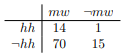
\includegraphics[width=0.25\linewidth]{Q2 Table.png}
\end{figure}

\begin{enumerate}[a)]
    \item $P(mw|hh)=\frac{14}{15}$\\ Counts irrelevant were 70 and 15, where Halaand did not score a hat-trick.
    \item $P(hh|mw)=\frac{14}{84}=\frac{1}{6}$\\Counts irrelevant were 1 and 15, where Man City did not win.
\end{enumerate}


\section{}
\begin{enumerate}[a)]
    \item $p(yng)=0.35\\p(rizz|yng)=0.01\\p(rizz|\neg yng)=0.001$\\
    $p(rizz|yng)\times p(yng)$\\
    $0.01 \times 0.35 = 0.0035$\\
    $p(rizz|\neg yng) \times p(\neg yng)$\\
    $0.001 \times (1-0.35) = 0.00065$\\
    $0.0035>0.00065$\\
    $yng$ is likelier.

    \item $p(yng)=0.05\\p(rizz|yng)=0.01\\p(rizz|\neg yng)=0.001$\\
    $p(rizz|yng)\times p(yng)$\\
    $0.01 \times 0.05 = 0.0005$\\
    $p(rizz|\neg yng) \times p(\neg yng)$\\
    $0.001 \times (1-0.05) = 0.00095$\\
    $0.0005<0.00095$\\
    $\neg yng$ is likelier.

    \item $p(yng)=0.05\\p(rizz|yng)=0.01\\p(rizz|\neg yng)=0.0005$\\
    $p(rizz|yng)\times p(yng)$\\
    $0.01 \times 0.05 = 0.0005$\\
    $p(rizz|\neg yng) \times p(\neg yng)$\\
    $0.0005 \times (1-0.05) = 0.000475$\\
    $0.0005>0.000475$\\
    $yng$ is likelier.
\end{enumerate}


\newpage
\section{}
\begin{figure}[h]
    \centering
    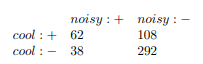
\includegraphics[width=0.5\linewidth]{Q4 Table.png}
\end{figure}
\[
p(cool:+) = \frac{170}{500} = \frac{17}{50}=0.34
\]
\[
p(cool:+|noisy:+) = \frac{62}{100} = \frac{31}{50}=0.64
\]
The formula for Independence: $P(A|B)=P(A)$. $0.34\neq 0.64$\\
$\therefore cool:+$ is not independent of $noisy:+$


\section{}
\begin{figure}[h]
    \centering
    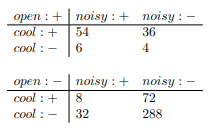
\includegraphics[width=0.4\linewidth]{Q5 Table.png}
\end{figure}
\[
p(cool:+|open:+)=\frac{90}{100}=0.9
\]
\[
p(cool:+|open:+,noisy:+)=\frac{54}{60}=0.9
\]
\[
p(cool:+|open:+)=p(cool:+|open:+,noisy:+)
\]
Conditional Independence: $P(X|Y,Z)=P(X|Y)$\\
$cool:+$ is conditionally independent of $noisy:+$ given $open:+$

\newpage
\section{}
H = $heads$, T = $tails$\\
$\theta_h$ is the probability of a coin flipping heads.\\
For $\theta_h = 0.1$\\
H H H T = $0.1 \times 0.1 \times 0.1 \times (1-0.1) = 0.0009$\\
For $\theta_h = 0.5$\\
$0.5 \times 0.5 \times 0.5 \times (1-0.5) = 0.0625$\\
For $\theta_h = 0.75$\\
$0.75 \times 0.75 \times 0.75 \times (1-0.75) = 0.1055$\\
For $\theta_h = 0.9$\\
$0.9 \times 0.9 \times 0.9 \times (1-0.9) = 0.0729$\\

\end{document}
